\subsection{Technologie 28nm FDSOI}

La fabrication de deux circuits s'est effectuée sur la technologie 28nm FDSOI de chez  \textit{ST Microelectronics}. Cette technologie est une technologie de pointe qui permet de fabriquer des circuits intégrés performants et qui, de par la présence de sa Back-Gate permet une grande flexibilité de fonctionnement. Aussi, la technologie FDSOI est connue pour sa robustesse aux radiations.



La Figure \ref{fig:coupeNMOS} est une vue en coupe d'un transistor LVT-NMOS, ou transistor NMOS à faible tension de seuil (Low-$V_{th}$-NMOS), fabriqué en technologie 28nm FD-SOI. En technologie FD-SOI, les transistors sont construits sur un isolant, ce qui permet au canal d’être entièrement déplété. Le silicium sous la couche d’isolation est dopé de type N dans le cas du LVT-NMOS et est appelé la grille arrière (back-gate).


\begin{figure}
    \centering
    \includegraphics[width=0.8\linewidth]{../Conf/ICECS2024/ICECS_Voltage_Reference/figures/LVT-NMOS.pdf}
    \caption{vue en coupe d’un transistor NMOS en technologie FD-SOI 28 nm \cite{cathelin_fully_2017}.}
    \label{fig:coupeNMOS}
\end{figure}

\subsubsection{Influence de la Back-Gate} 
La technologie FDSOI est une technologie qui permet de contrôler la tension de seuil des transistors en agissant sur la tension de la Back-Gate.  En effet, en appliquant une tension sur la Back-Gate, on crée un champ électrique qui va modifier la concentration de porteurs dans le canal du transistor. Cette modification de concentration de porteurs va modifier la tension de seuil du transistor. La techn FDSOI permet donc un controle fin de la tension de seuil et de la performance des transistors au travers d'une tension.

\begin{figure}
    \centering
    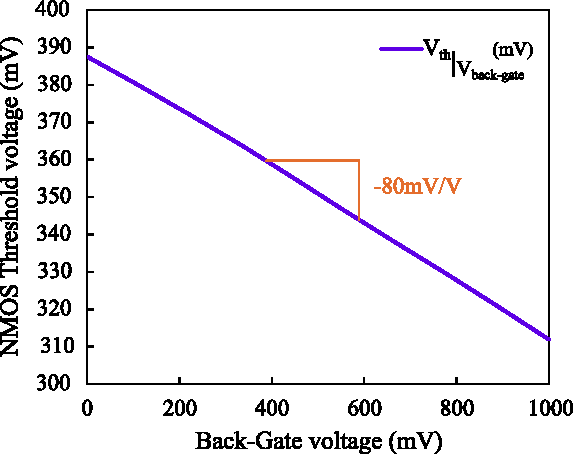
\includegraphics[width=0.7\textwidth]{../Conf/ICECS2024/ICECS_Voltage_Reference/figures/Vt(Vbb).pdf}
    \caption{Evolution de la tension de seuil en fonction de la tension de la Back-Gate}
    \label{fig:Vt(Vbb)}
\end{figure}

La tensions de seuil variant linéairement avec la tension de la Back-Gate, il est possible de determiner l'équation de la tension de seuil en fonction de la tension de la Back-Gate. Cette équation est donnée par l'équation \ref{eq:Vt(Vbb)}.

\begin{equation}
    V_{th}(T) = \beta V_{BB} + V_{th_0}\hspace*{0.3cm}(V)
    \label{eq:Vt(Vbb)}
\end{equation}
Avec:

\begin{itemize}
    \item $\beta$ : la sensibilité de la tension de seuil à la tension de la Back-Gate en $mV/V$, ici: $\beta=80mV/V$.
    \item $V_{BB}$ : la tension de la Back-Gate.
\end{itemize}
